\section{Beschreibung der Anwendung}
\label{sec:beschreibung}
\subsection{Admindialog}
Im \textit{Admindialog} können Administratoren Bewohner, Wohngruppen/-heime und Mitarbeiter verwalten.
\begin{figure*}[h]
	\begin{center}
		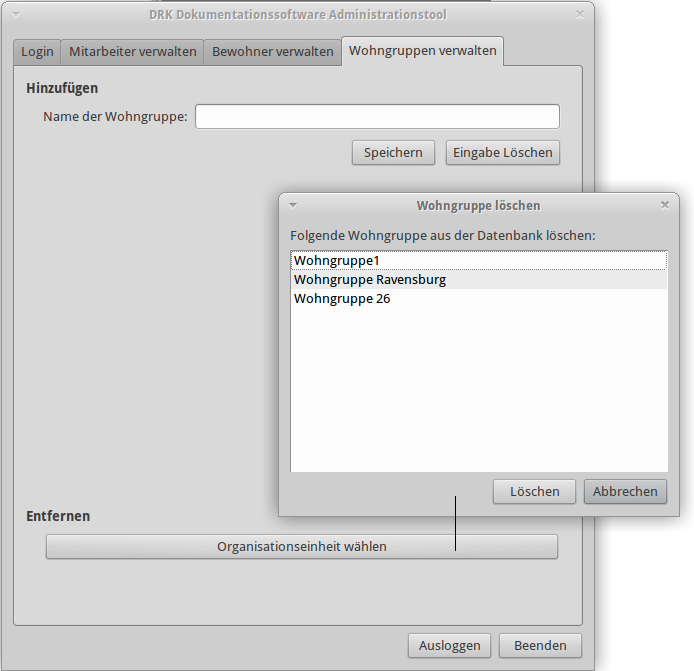
\includegraphics[keepaspectratio=true, width=0.85\textwidth]{pics/admin3.png}
		\caption{Graphen eines Interfaces}
		\label{Admindialog Mitarbeiter erstellen}
	\end{center}
\end{figure*}
\FloatBarrier
\noindent
Hier werden Wohngruppen erstellt, diese dienen als Gruppierung für sowohl Bewohner, als auch für Mitarbeiter.
\newpage
\noindent
Bewohner werden mit einer Bewohnernummer, Vor-/Nachnamen und ihrer Wohngruppe  erstellt. 
\begin{figure*}[h]
	\begin{center}
		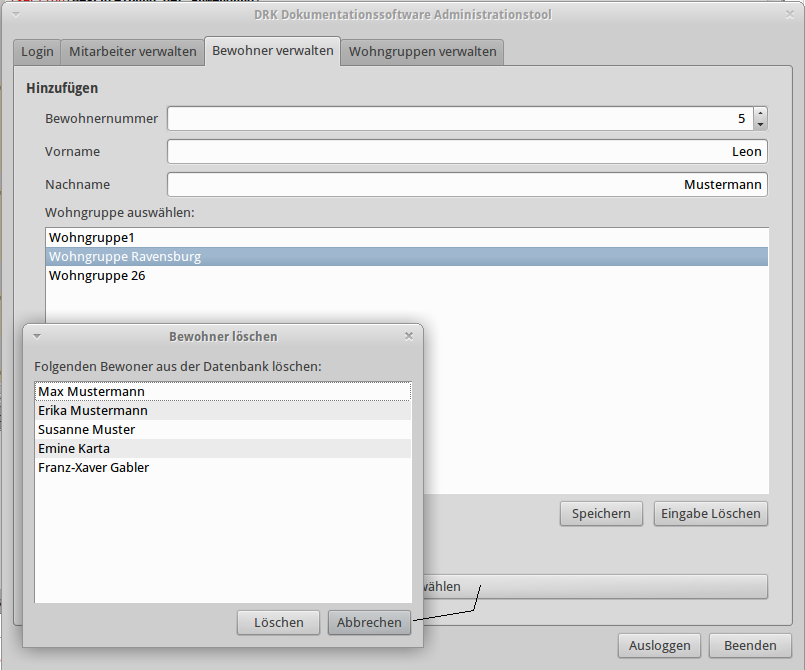
\includegraphics[keepaspectratio=true, width=0.85\textwidth]{pics/admin2.png}
		\caption{Graphen eines Interfaces}
		\label{Admindialog Bewohner}
	\end{center}
\end{figure*}
\FloatBarrier
\noindent
Restliche Informationen werden im Client von zugewiesenen Bezugsbetreuern ausgefüllt.
\newpage
\noindent
Mitarbeiter werden mit Login sowie einigen persönlichen Daten, Name und Kontaktmöglichkeiten, sowie ihrer Berechtigung erstellt. Es ist darauf zu achten das jedem Mitarbeiter beim erstellen mindestens eine Wohngruppe zugeordnet werden muss, die er betreut. Er kann allerdings natürlich auch für mehrere Wohngruppen zuständig sein und auch der Bezugsbetreuer für Bewohner sein.
\begin{figure*}[h]
	\begin{center}
		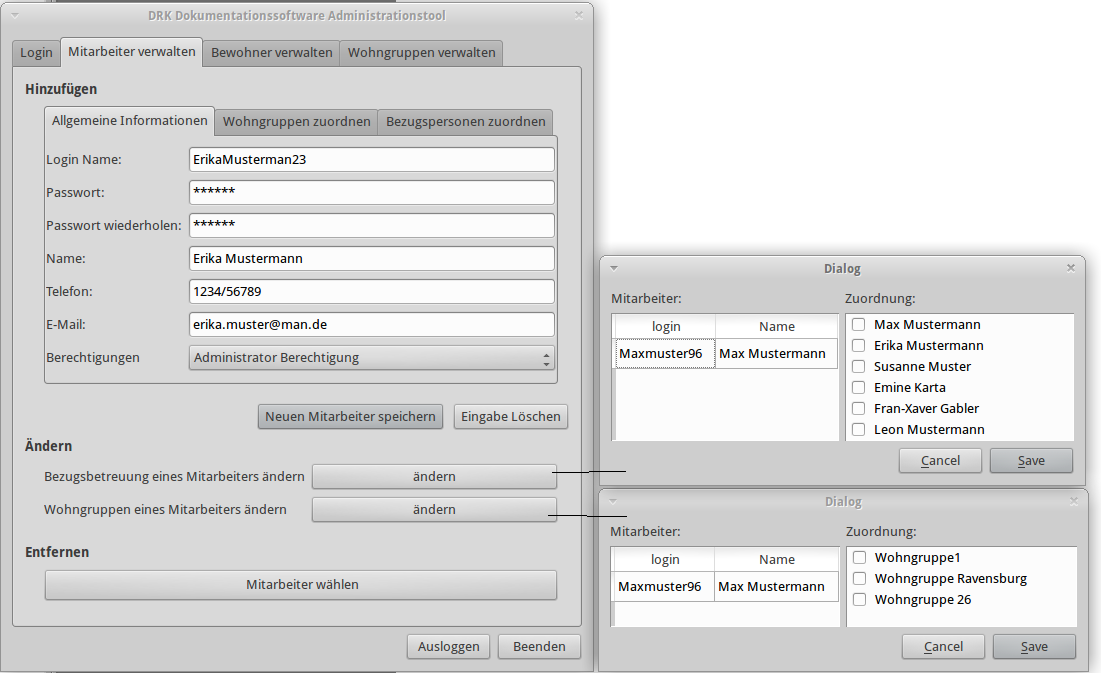
\includegraphics[keepaspectratio=true, width=0.85\textwidth]{pics/admin1.png}
		\caption{Graphen eines Interfaces}
		\label{Admindialog Bewohner}
	\end{center}
\end{figure*}
\FloatBarrier
\noindent
Mitarbeiter die keine Administratorenrechte haben können nur Informationen von Bewohner in ihrer Wohngruppe einsehen und nur von Bewohner deren Bezugsbetreuer sie sind verändern.
\subsection{Client}

\subsection{Lokalisierung}
Sowohl der AdminDialog wie auch die \EBP sind komplett lokalisierbar. Qt stellt dafür einen einfachen Mechanismus zur Verfügung. Jeder zu lokalisierende String wird dabei von eimem Makro umschlossen. Das 
\subsection{Erstellen der Anwendung}
\subsubsection{Abhängigkeiten}
\paragraph{Zur Laufzeit:}
\begin{itemize}
	\item \textbf{odb} - ODB Laufzeitbibliothek
	\item \textbf{odb-mysql} - MySQL Backend für ODB
	\item \textbf{odb-qt} - QT integration für ODB
	\item \textbf{qt} - QT Framework
\end{itemize}
\paragraph{Zur Compilezeit:}
\begin{itemize}
	\item \textbf{CMake} - Buildsystem
	\item \textbf{ODB Toolchain} - Enthält den Precompiler
	\item \textbf{GCC} - GNU Compiler Collection
\end{itemize}
\subsubsection{Kompilieren der Quellen}
Die komplette Anwendung kann im Wurzelverzeichnis des Projekts gebaut werden:\\
\begin{lstlisting}
$ cmake .
\end{lstlisting}
Generiert das benötigte Makefile.\\
Ist dies erfolgreich abgeschlossen, wird mit\\
\begin{lstlisting}
$ make
\end{lstlisting}
der eignetliche Kompiliervorgang gestartet.\\
\subsubsection{Vorbereiten der Datenbank}
Um die Datenbank zu initialisieren befindet sich ein Shell-Script im EBPdb Verzeichnis:\\
\begin{lstlisting}
$ ./initDB.sh -u root -p "DATENBAKNAME"
\end{lstlisting}
